\begin{enumerate}
\item Le nombre de manières de colorier un graphe est le produit des nombres de façons de colorier chaque arc.
\begin{itemize}
\item Si le graphe $G$ est complet, on aura $k$ couleurs possibles pour le premier sommet, $(k-1)$ pour le deuxième, etc\ldots (Le graphe G étant complet, la couleur du premier sommet est nécessairement exclu des autres sommets)

Le $n$\^{ième} sommet pourra être colorié de $k-(n-1)$ manières. D'où :
\[ P_{K_n}(k)=\prod_{i=0}^{n-1}(k-i) \]

\item Si $G$ est vide, la coloration d'un sommet ne contraint pas la coloration des autres sommets. On obtient alors :
\[ P_{\overline{K_n}}(k)=k^n \]
\end{itemize}
\item $\chi(G)$ étant, par définition, le nombre minimum de couleurs nécessaires pour colorier $G$, si $k < \chi(G)$ alors le graphe $G$ ne peut pas être colorié par $k$ couleurs. Si $k \geq \chi(G)$ alors il doit y avoir au moins une manière de colorier $G$, celui utilisant $\chi(G)$ couleurs.

On a donc :
\begin{displaymath}
	P_G(k) \left\{ \begin{array}{ll}
	=0 & \textrm{si $k < \chi(G)$} \\
	\geq 1 & \textrm{sinon}
	\end{array} \right.
\end{displaymath}

\item Montrons d'aboard que la propriété est vraie pour tout graphe complet $K_n$. Pour commencer on remarque que, pour tout arrête $e$:

\begin{itemize}
\item $K_{n\backslash e}$ est exactement $K_{n-1}$, et donc: 

\[ P_{K_n\backslash e}(k) = P_{K_{n-1}} = \prod_{i=0}^{n-2}(k-i) \]


\item Soit $e = (a,b)$. On peut supposer (sans perte de généralité) que $b$ est considéré en dernier lors de la coloration de $K_n$, donc qu'il lui reste $k-(n-1)$ couleurs. Pour colorier $K_{n-e}$ on aura un choix de plus pour lui, à savoir la couleur de $a$, donc $k-(n-2)$ en totale. De ce fait:

\[ P_{K_n-e}(k) = P_{K_{n-1}}(k)(k-(n-2)) = (\prod_{i=0}^{n-2}(k-i))(k-(n-2)) \]
\end{itemize}

On a donc très clairement:
\begin{eqnarray*}
P_{K_n-e}(k) -  P_{K_n\backslash e}(k) &=& (\prod_{i=0}^{n-2}(k-i))(k-(n-2)) - \prod_{i=0}^{n-2}(k-i)\\
&=& \prod_{i=0}^{n-2}(k-i)(k-(n-1))\\
&=& \prod_{i=0}^{n-1}(k-i)\\
&=& P_{K_n}(k)
\end{eqnarray*}
Tout graphe de rang $n$ pouvant se générer à partir de $K_n$ (en enlevant des arrêtes) on cherchera à prouver que la suppression d'arrête conserve notre propriété. Autrement dit on aimerait montrer que pour tout graphe $G$ et tout arrête $a$ de celui-ci:

\begin{eqnarray*}
&&P_G(k) = P_{G-e}(k) - P_{G \backslash e}(k) \\
&\Rightarrow&  P_{G-a}(k) = P_{G-e-a}(k) - P_{G \backslash e-a}(k)
\end{eqnarray*}

On supposera évidemment que $a$ et $e$ sont distinctes. 

TODO FINISH

\item Soit $H$ un prédicat tel que :
\begin{displaymath}
	H(m) \left\{ \begin{array}{ll}
	\top & \textrm{si $\forall$ $G$, graphe de $m$ arrêtes ou moins, $P_G(k)$ est polynomiale.} \\
	\bot & \textrm{sinon.}
	\end{array} \right.
\end{displaymath} 
\begin{itemize} 
\item Nous rappellons que $P_{\overline{K_n}}(k)=k^n$, donc $H(0)$ est vraie. 
\item Supposons $\exists m \in \mathbb{N}$ $|$ $H(m)$ l'est également. Soit $G_{m+1}$ un graphe à $m+1$ arrêtes:

\[ P_{G_{m+1}} = P_{G_{m+1}-e} - P_{G_{m+1} \backslash e} \]

Clairement $P_{G_{m+1}-e}$ et $P_{G_{m+1} \backslash e}$ ont $(m+1)-1 = m$ arrêtes. Or par hypothèse de recurrence $H(m)$ est vraie,
$P_{G_{m+1}}$ est la différence entre deux polynomiales, donc est polynomiale lui-même. On a donc $H(m+1)$.
\item On vient de montrer $H(0) \wedge (H(m) \Rightarrow H(m+1))$. Par récurrence on a donc $H(m) \forall m \in \mathbb{N}$. 

\end{itemize} 



\item Utilisons la formule trouvée au point précédent, et admettons que pour $P_n$ une chaîne de taille $n$ on a :
\[ P_n(k) = k(k-1)^{n-1} \]

Prenons $A$ le graphe initial :
\begin{eqnarray*}
P_A(k) & = & P_B(k) - P_C(k) \\
&=& \big(P_D(k)-P_E(k)\big)-\big(P_F(k)-P_{P_3}(k)\big)\\
&=& \Big[\big(P_{P_5}(k)-P_{P_4}(k)\big)-\big(P_{P_4}(k)-P_{P_3}(k)\big)\Big]-\Big[\big(P_{P_4}(k)-P_{K_3}(k)\big)-P_{P_3}(k)\Big]\\
&=& P_{P_5}(k)+2P_{P_3}(k)-P_{K_3}(k)+3P_{P_4}(k)\\
&=& k(k-1)^4 +2k(k-1)^2+k(k-1)(k-2)-3(k-1)^3 \\
&=& k(k-1)\big[(k-1)^3+z(k-1)+(k-z)-3(k-1)^2\big]\\
&=& (k^2-k)\Big[(k-1)^2\big((k-1)-3\big)+3k -4 \Big]\\
&=& (k^2-k)[k^3-6k^2+12k-8]\\
&=& k^5-7k^4+18k^3-20k^3+8k
\end{eqnarray*}
Où :

$A$ : \raisebox{-0.5\height}{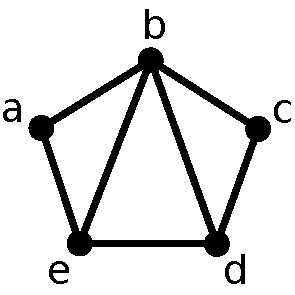
\includegraphics[width=2cm]{files/gAex1.pdf}}

\begin{tabular}{llcll}
$B = A-(e,d) $ : & \raisebox{-0.5\height}{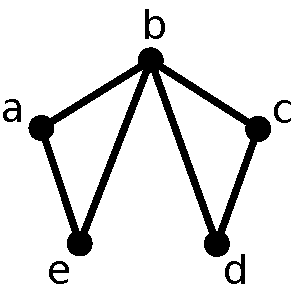
\includegraphics[width=2cm]{files/gBex1.pdf}} & et & $C = A\backslash(e,d)$ : & \raisebox{-0.5\height}{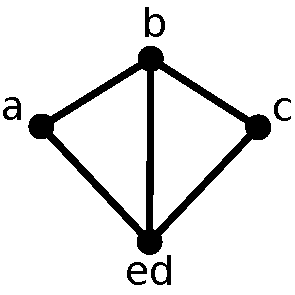
\includegraphics[width=2cm]{files/gCex1.pdf}} \\
$D = C-(a,b)$ : & \raisebox{-0.5\height}{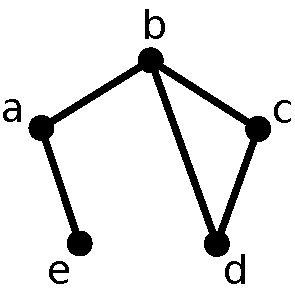
\includegraphics[width=2cm]{files/gDex1.pdf}} & et & $E = C\backslash(e,b)$ : & \raisebox{-0.5\height}{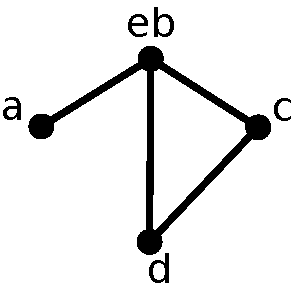
\includegraphics[width=2cm]{files/gEex1.pdf}} \\
$F = C-(b,ed)$ : & \raisebox{-0.5\height}{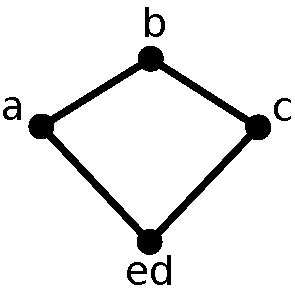
\includegraphics[width=2cm]{files/gFex1.pdf}}& et & $C \backslash(b,ed) = P_3$ : & \raisebox{-0.5\height}{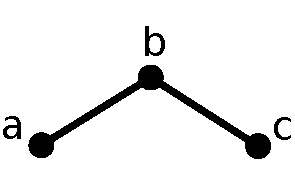
\includegraphics[width=2cm]{files/gC-ex1.pdf}}
\end{tabular}

\item TODO coéfficient de $k^n$ est 1, alternating - and + etc 


\item

\end{enumerate}